\chapter{Implémentation}
Les fonctions demandées dans le sujet ont été implémentées, avec quelques spécificités selon la compréhension du sujet. Par exemple, certains vérifications ont été ajoutées (vérification qu'une ludothèque ou qu'un jeu n'est pas \lstinline{NULL}). A l'inverse, certaines vérifications sur les entrées utilisateurs n'ont pas été faites (on ne vérifie pas que lorsqu'un entier est attendu, l'utilisateur a bien tapé un entier).

\section{Programme principal}
Le programme principal affiche à l'utilisateur un menu qui lui donne le choix parmi \textbf{6 possibilités} :
\begin{enumerate}
  \item Créer une ludothèque
  \item Afficher une ludothèque
  \item Ajouter un jeu dans la ludothèque en saisissant ses caractéristiques
  \item Effectuer une recherche de jeu à partir de critères saisis par l’utilisateur
  \item Créer 2 ludothèques, les afficher, les fusionner puis afficher la nouvelle ludothèque
  \item Quitter le programme
\end{enumerate}
L'utilisateur tape au clavier le numéro de son choix. Un \lstinline{switch} permet d'effectuer les actions correspondantes à l'entrée clavier.
\textcode{main.c}
\begin{lstlisting}
// ...
afficherMenu();
while((inputUser = getchar()) != '6') {
  // ...
  switch(inputUser) {
    case '1':
        // ...
        break;
    case '2':
        // ...
        break;
    case '3':
        // ...
        break;
    case '4':
        // ...
        break;
    case '5':
        // ...
        break;
    default:
        printf("Mauvaise entrée. Veuillez taper 1, 2, 3, 4, 5 ou 6.\n");
        continue; // On recommence la boucle while
  }
  // ...
  afficherMenu();
}
// ...
\end{lstlisting}
Une boucle \lstinline{while} permet d'afficher à nouveau le menu après être sorti du \lstinline{switch}. L'invariant de boucle est \textbf{\lstinline{(inputUser = getchar()) !='6'}}.

\section{Gestion d'une ludothèque}
La structure d'une ludothèque a été définie dans le fichier \textit{ludotheque.h} :
\textcode{ludotheque.h}
\begin{lstlisting}
struct ludotheque {
    int nb_jeu;
    t_jeu *debut;
};
\end{lstlisting}

\subsection{Fonction \lstinline{ajouter_jeu}}
La fonction \lstinline{int ajouter_jeu(t_ludotheque* ludo, t_jeu* j);} permet d'ajouter un jeu même si celui-ci est déjà présent dans l'actuelle ludothèque, en maintenant la ludothèque triée selon le nom des jeux. \textbf{Il n'était pas précisé dans le sujet si les doublons devaient être évités pour cette fonction}. Lors de la fusion de 2 ludothèques, une vérification est faite pour ne pas ajouter deux fois un jeu présent dans dans les 2 ludothèques (fonction vue en TD).

\medskip

Voici une autre fonction qui permet d'ajouter un jeu à une ludothèque en évitant les doublons, (\textbf{cette fonction n'est pas dans notre code source}):
\textcode{Fonction \lstinline{ajouter_jeu_no_doublon}}
\begin{lstlisting}
int ajouter_jeu_no_doublon(t_ludotheque* ludo, t_jeu* j) {
    if (j==NULL || ludo == NULL) return 0;
    t_jeu* tete = ludo->debut;
    if (tete == NULL || strcmp(j->nom,tete->nom) < 0) {
        j->suivant = ludo->debut;
        ludo->debut = j;
    }
    else {
        while(tete->suivant != NULL && strcmp(j->nom,tete->suivant->nom) > 0) {
            tete = tete->suivant;
        }
        if (tete->suivant != NULL && strcmp(j->nom,tete->suivant->nom) == 0) {
            return 0; // Le jeu est déjà présent (même nom)
        }
        // Le jeu n'est pas présent, on l'ajoute
        j->suivant = tete->suivant;
        tete->suivant = j;
    }
    return 1;
}
\end{lstlisting}

\subsection{Fonction ajoutée}
En plus des fonctions demandées dans le sujet, nous avons ajouté la fonction
\textcode{ludotheque.h}
\begin{lstlisting}
  t_ludotheque* saisir_requete(t_ludotheque *ludo);
\end{lstlisting}
pour obtenir un code mieux organisé. Elle permet de demander à l'utilisateur d'entrer les différents paramètres de sa requête. Cette fonction appelle ensuite la fonction
\begin{lstlisting}
  t_ludotheque* requete_jeu(t_ludotheque *ludo, genre_jeu genre, int nbJoueurs, int duree);
\end{lstlisting}
demandée dans le sujet du TP.

\section{Gestion des jeux}
L'énumation des genre ainsi que la structure d'un jeu ont été définis dans le fichier \textit{jeu.h} :
\textcode{jeu.h}
\begin{lstlisting}
typedef enum genre {
    PLATEAU, RPG, COOPERATIF, AMBIANCE, HASARD
} genre_jeu;

typedef struct jeu {
    char *nom;
    genre_jeu genre;
    int nbJoueurMin;
    int nbJoueurMax;
    int duree;
    struct jeu *suivant;
} t_jeu;
\end{lstlisting}

\subsection{Fonctions ajoutées}
Nous avons ajouté trois fonctions destinées à éviter de répéter beaucoup de code à divers endroits :
\textcode{jeu.h}
\begin{lstlisting}
t_jeu* saisir_jeu();

char *stringFromGenre(enum genre g);

genre_jeu genreFromString(char *str);
\end{lstlisting}

La première fonction permet de demander à un utilisateur les paramètres d'un jeu, en vue de créer ce jeu (la fonction retourne un pointeur de jeu).

\medskip

Les deux fonctions suivantes permettent de manipuler une \lstinline{enum} sous forme de \lstinline{string} et inversement de manière très simple, cela est plus pratique pour l'affichage sur la console.

\medskip

Nous avons arbitrairement décidé pour la dernière fonction que si le paramètre \lstinline{char *str} ne correspondait pas à un genre de jeu qui existe, alors nous retournerions le type \lstinline{HASARD}. De plus, nous avons utilisé la fonction \lstinline{strcasecmp} grâce à \lstinline{#include <strings.h>} pour pouvoir comparer des \lstinline{strings} sans tenir compte de la casse. Nous aurions pu utiliser la fonction \lstinline{strcmp} qui, elle, tient compte de la casse.


\chapter{Capture d'écran}
Voici un aperçu de notre programme :
\begin{figure}[!h]
   \centering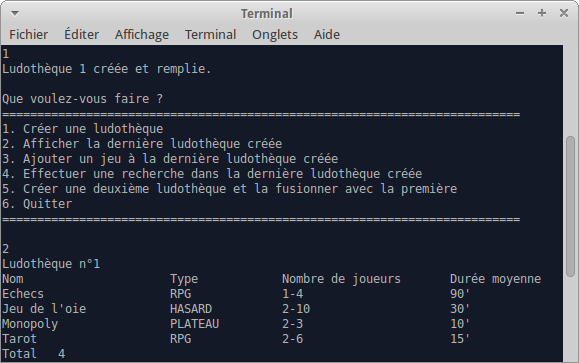
\includegraphics[width=0.8\textwidth]{sample.png}
   \caption{L'utilisateur a choisi 1 puis 2 dans le menu d'options}
\end{figure}